\chapter{Theoretische Einführungen}

\section{Oberflächenplasmonenpolaritonen}~\label{sec:spps}
Oberflächenplasmonenpolaritonen (engl. surface plasmon polaritons, SPPs)
sind kollektive Oszillationen des Elektronengases, welche sich entlang der Grenzfläche
zwischen Leiter und Dielektrikum ausbreiten.\cite{plasmonics}
Sie entstehen durch Anregungen des Elektronengases in metallischen Materialien.
Eine Anregung kann z.B. durch Licht geschehen.

\begin{wrapfigure}{l}{5cm}
    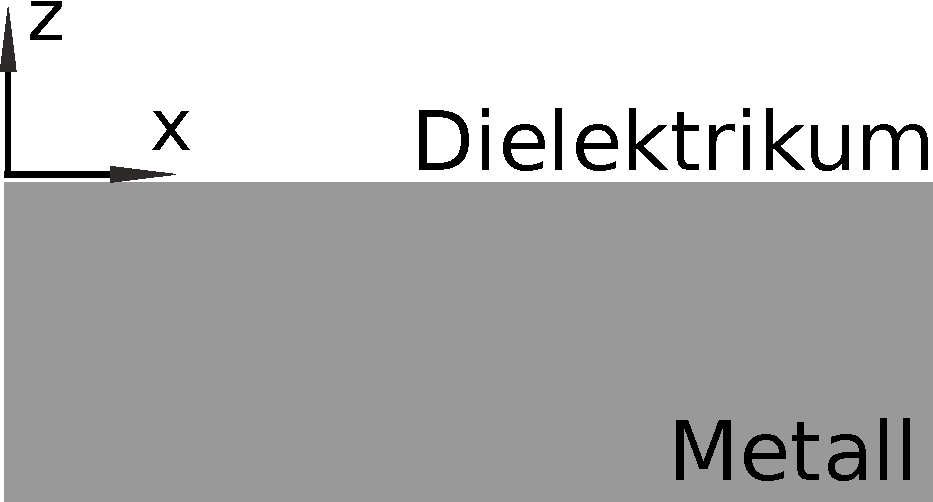
\includegraphics[width=4.5cm]{./Plots/leiter_und_nichtleiter.pdf}
    \caption{Darstellung einer Grenzfläche zwischen Leiter und Dielektrikum an welcher 
    SPPs entstehen können. Zur Vereinfachung hier eine Ausbreitung in x-Richtung angenommen.\\}
    \label{fig:kasten}
\end{wrapfigure}
\FloatBarrier

Plasmonen sind Quasiteilchen. 
Also ein Phänomen was ein Teilchencharakter besitzt bzw. einem ein solcher zugeordnet werden kann. 
Eine Eigenschaft der SPPs ist ihr evaneszentes Verhalten bezogen auf das
durchdringen der Grenzfläche. 
Das bedeutet das die Amplitude der Wellenfunktion exponentiell beim durchdringen abfällt.
Der theoretische Zugang zu SPPs gelingt über die Verwendung der Maxwellgleichungen, welche dazu
genutzt werden um die Helmholzgleichung 
\begin{equation}
    \nabla^2 \vec{E} + k^2_0 \, \epsilon \, \vec{E} = 0
    \label{eq:helm}
\end{equation}
zu formulieren. 
Dabei steht $\vec{E}$ für den elektrischen Feldvektor, $k_0 = \sfrac{\omega}{c}$ 
für der Wellenvektor und $\epsilon$ für die Permittivität.
Aus Gleichung~\ref{eq:helm} lassen sich im folgenden mehrere gekoppelte Differentialgleichungen
herleiten, welche wiederrum in 2 Gleichungen überführt werden, die Transversalelektrischewellen (TE) und 
Transversalmagnetischewellen (TM) beschreiben.
Die Besonderheit bei TM-Wellen und TE-Wellen ist das 
die Komponente der Amplitude in Ausbreitungsrichtung verschwindet.

Werden TE-Wellen betrachtet sorgen die Randbedingungen an der Grenzfläche
dafür das die Amplitude insgesamt verschwindet.\cite{plasmonics} 
Aus diesem Grund gibt es nur SPPs, welche durch TM-Moden beschrieben werden. 
Die Dispersionsrelation für eine propagierende Welle von SPPs lautet
\begin{equation}
    k_\text{spp} = k_0 \sqrt{\frac{\epsilon_1 \,\epsilon_2}{\epsilon_1 + \epsilon_2}}.
    \label{eq:disp}
\end{equation}
Hierbei sind $\epsilon_1$ und $\epsilon_2$ die unterschiedlichen Permittivitäten des Leiters und
des Dielektrikums.
Wie bereits genannt lassen sich SPPs durch Licht anregen.
Um dies zu realisieren muss\footnote{Es gibt auch noch andere Möglichkeiten,
die in dieser Arbeit aber nicht weiter thematisiert werden.} sich ein metallisches Gitter 
(z.B. aus Gold) auf der Oberfläche befinden.

\begin{figure}
    \centering
    \begin{subfigure}{0.5\textwidth}
        \centering
        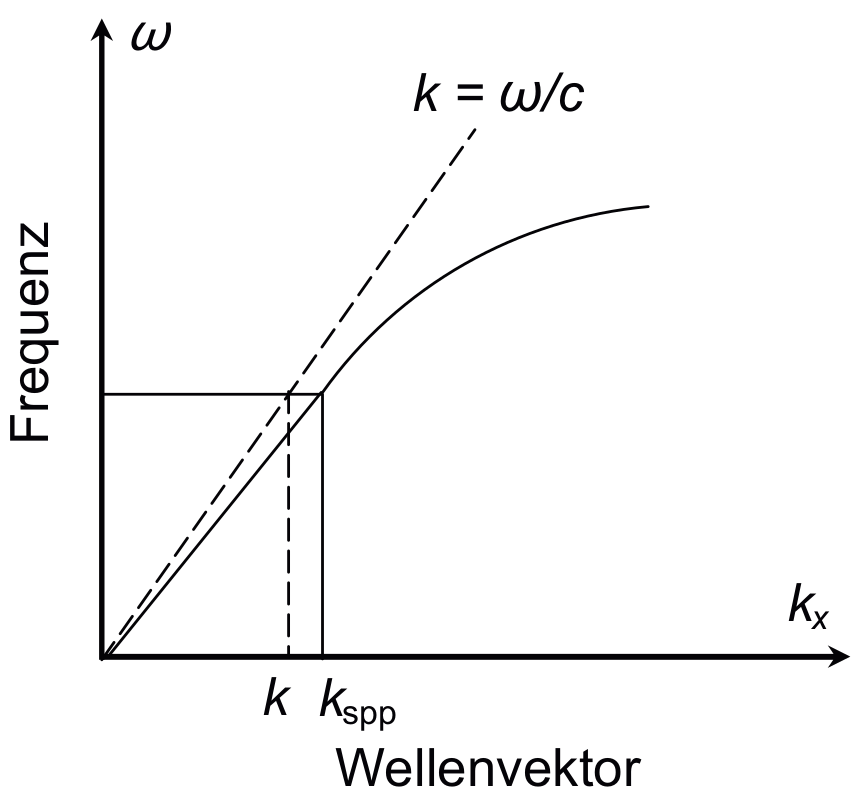
\includegraphics[width=5.5cm]{./Plots/disp.png}
        \caption{Darstellung der Dispersionsrelation von einer SPP und der eines freien Photons.
        Es existiert für keinen Wert von $k_x$ ein Schnittpunkt der Dispersionen. \cite{disp}}
        \label{fig:disp}
    \end{subfigure}
    \begin{subfigure}{0.5\textwidth}
        \centering
        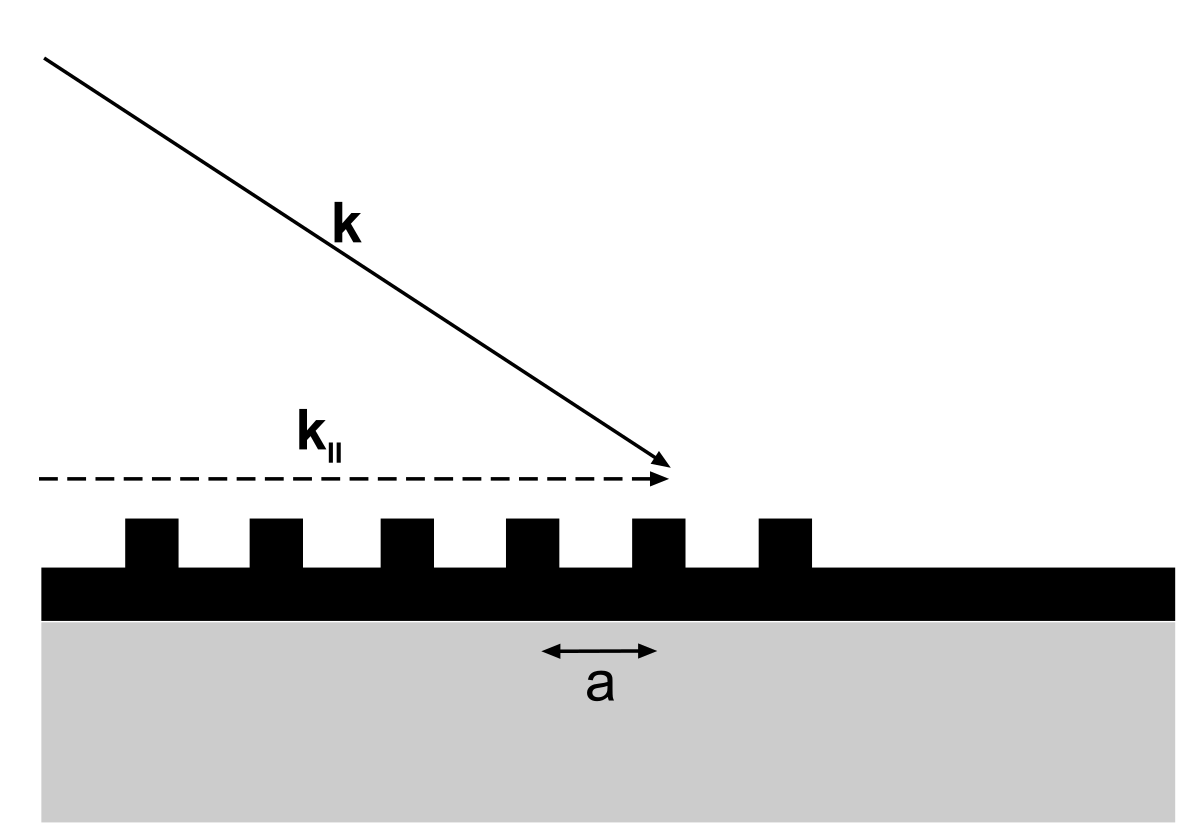
\includegraphics[width=5.5cm]{./Plots/gitter.png}
        \caption{Periodische Gitterstruktur welche sich auf einer Probenoberfläche befindet. 
        Diese ist notwendig damit die Plasmonen in der Lage sind an Photonen zu koppeln.\cite{disp} }
        \label{fig:gitter}
    \end{subfigure}
    \caption{Darstellung des Dispersionverlauf einer SPP und eines periodischen Goldgitters auf einer Probenoberfläche.}
    \label{fig:disp_und_gitter}
\end{figure}
\FloatBarrier

In Abbildung~\ref{fig:disp} ist die Dispersionsrelation für eine SPP und ein freies Photon zu sehen. 
Da es zwischen dem Verlauf von $k_\text{spp}$ und $k$ keinen Schnittpunkt gibt, kann
in diesem Fall keine Anregung eines SPPs erfolgen. 
Ein Schnittpunkt würde  einer energie- und impulserhaltenden Anregung entsprechen.
Der Prozess der Anregung eines SPPs ist auch umgekehrt möglich.

Befindet sich ein Goldgitter (vgl. Abbildung~\ref{fig:gitter}) 
mit Periodizität $a$ auf der Oberfläche so lässt sich 
ein SPP immer dann anregen wenn die Bedingung
\begin{equation}
    k_\text{SPP} = k \sin(\theta) \pm m \, G, \quad  m \in \mathbb{N}^+
\end{equation}
erfüllt ist.
Das SPP nimmt also nur einen Impuls in paralleler Richtung zur Oberfläche unter dem Winkel $\theta$ auf.
Es können beliebig viele verschiedene Ordnungen von
reziproken Gittervektoren $G = \sfrac{2 \, \pi}{a}$ hinzuaddiert werden.

\section{Große Zeemanaufspaltung}\label{sec:Große Zeemanaufspaltung}
Der Zeeman-Effekt beschreibt im allgemeinen das Phänomen der Aufspaltung von 
Energieniveaus beim anlegen eines äußeren Magnetfelds. 
Historisch gesehen wird auch oftmals anstelle von Energieniveaus von Spektrallinien gesprochen, 
da diese zuerst experimentell nachgewiesen worden sind.
Das Bändermodell in einem Festkörper ist von der Zeemanaufspaltung ebenfalls betroffen.
Im Falle der in der dieser Arbeit verwendeten semimagnetischen Halbleiter ist die Zeemanaufspaltung
sehr groß.\cite{zeeman}

In Abbildung~\ref{fig:zeeman} ist die Zeemanaufspaltung der im Experiment verwendeten Probe schematisch dargestellt.
Die Zeemanaufspaltung ist durch ein Magnetfeld entstanden, welches sich in Voigt-Geometrie befindet.
\begin{figure}
    \centering
    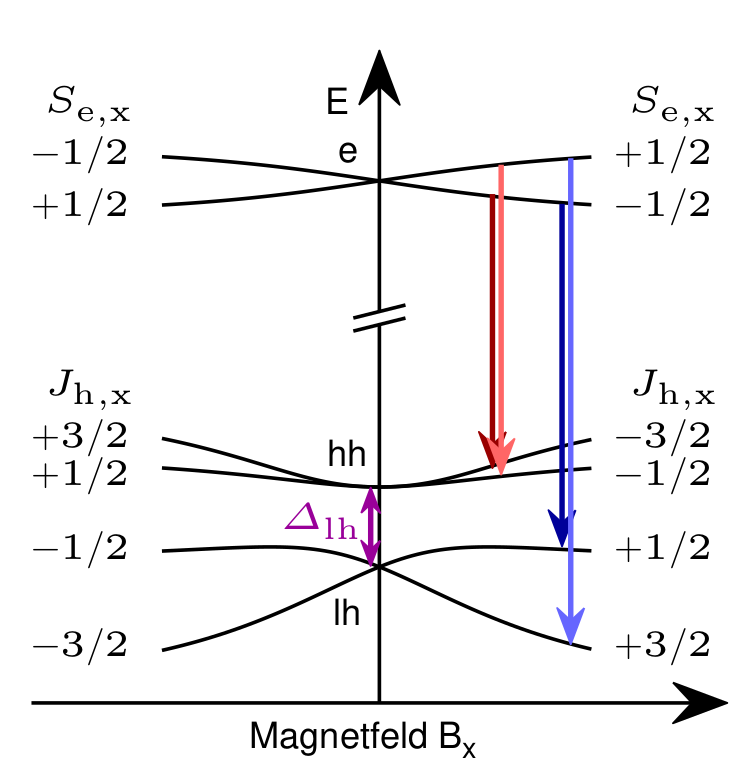
\includegraphics[scale=0.25]{./Plots/zeeman.png}
    \caption{Zeemanaufspaltung der unterschiedlichen Energiebänder bei äußerem Magnetfeld in Voigt-Geometrie.\cite{felix}
    Voigt-Geometrie bedeutet, dass die Magnetfeldlinien parallel zu Probenoberfläche verlaufen}
    \label{fig:zeeman}
\end{figure}
\FloatBarrier

Wird ein äußeres Magnetfelds angelegt, spaltet sich das Leichtloch~(engl. light hole, lh ) 
und das Schwerloch~(engl. heavy hole, hh) in jeweils 2 neue Niveaus auf.
Die Aufspaltung des Leichtlochs ist größer als die des Schwerlochs.
Ebenfalls entstehen 2 neue Niveaus des Leitungsbandes.
Die erlaubten optischen Übergänge und die dabei entstehenden unterschiedlichen 
Polarisationen des Lichts (beim Übergang) sind durch die Übergangsregeln festgelegt.
Bei den beiden blauen Übergängen in Abbildung~\ref{fig:zeeman} handelt
es sich um eine linkszirkulare Polarisation, also $\sigma^-$.
Bei den roten um eine rechtszirkulare, also  $\sigma^+$. 
Ein $\sigma$-Übergang bedeutet das ein $\Delta m$ der magnetischen Quantenzahl von 
$\pm 1$ angenommen wird.
Wird ein negatives Magnetfeld (linke Seite in Abbildung~\ref{fig:zeeman}) betrachtet,
dann ändern sich die Polarisationen von links- nach rechtszirkular und umgekehrt.
So ist beispielsweise, für negatives Magnetfeld, der ein Übergang von $S_\text{e,x} = \sfrac{-1}{2}$
nach $J_\text{h,x} = \sfrac{1}{2}$ linkszirkular Polarisiert.

Bei der im Experiment verwendeten Probe existiert ein großes $\Delta_\text{lh}$ (vgl. Abbildung~\ref{fig:zeeman}).
Dies ist wegen der in z-Richtung herrschenden starken räumlichen Einschränkung (engl. confinement) im Quantentopf der Fall.
Die Größe $\Delta_\text{lh}$ beschreibt die Differenz zwischen Leichtloch und Schwerloch und ist
in diesem Fall $\Delta_\text{lh}= \SI{20}{\milli\eV}$ groß.
Dies hat zur Folge, dass die Übergange zwischen Leitungsband und Schwerlochband deutlich
wahrscheinlicher sind als zwischen Leitungsband und Leichtlochband. Somit entstehen quasi nur 
Übergange in das Schwerlochband.

%Bei den beschriebenen $\sigma$ Übergängen handelt es sich Streng genome
%ellipstisch pola ? oder 

\section{Magnetisch kontrollierte direktionale Lichtemission}\label{sec:pl}
Die magnetisch kontrollierte direktionale Lichtemission
beschreibt wie mit Hilfe eines angelegten äußeren Magnetfelds, die Lichtemission
einer Halbleiterprobe gesteuert/geführt werden kann.
Das Prinzip ist, dass die Umpolung des Magnetfelds eine Änderung des SPP-Impulses zurfolge hat 
und dadurch die Lichtemission in eine andere Raumrichtung verläuft.
\begin{figure}
    \centering
    \includegraphics[scale=0.75]{./Plots/probe_komplett.pdf}
    \caption{Im Experiment verwendeter Probenkörper (vgl. Abbildung~\ref{fig:probe}).
    In den verschiedenen Schichten des Hybridhalbleiters entstehen Exzitonen und SPPs 
    welche miteinander koppeln. Am Goldgitter der Oberfläche wird das PL (roter Pfeil)
    emittiert.    
    Das angelegte Magnetfeld ist homogen und verläuft entlang der x-Achse der Probe.
    Die Richtung des Magnetfelds ist umkehrbar.}
    \label{fig:komplett}
\end{figure}
\FloatBarrier

Die in Abbildung~\ref{fig:komplett} zu sehende Halbeiterprobe befindet sich 
in einem homogenen Magnetfeld entlang der x-Achse.
Mit Hilfe eines Lasers werden im Quantentopf der Probe Exzitonen erzeugt.
Exzitonen beschreiben Quasiteilchen welche von einem Elektron-Loch-Paar gebildet werden.
Elektron-Loch-Paare entstehen z.B. wenn ein Laser 
Elektronen aus dem Valenzband in das Leitungsband hebt.\cite{jens}

Bei einem Magnetfeld von $B_{x} = 0$ können nur Exzitonen in der x-y-Ebene entstehen (vgl. Abbildung~\ref{fig:exziton}).\cite{felix}
Diese Exzitonen besitzen unterschiedliche zirkulare Polarisation, aber sehr dominierend diese, welche bei 
Schwerloch-Übergängen entstehen (vgl.Abbildung~\ref{sec:Große Zeemanaufspaltung}).

% ich dachte daes hh und lh auch bei b=0 gibt ja gibt es vgl bild TODO eig erledigt

Wird das Magnetfeld $B_{x} \neq 0 $ so werden die Exzitonen anteilig um die x-Achse gekippt(vgl. Abbildung~\ref{fig:exziton}).
Das hat zur Folge das die Exzitonen in der y-z-Ebene elliptisch polarisiert erscheinen. 
Für weitere Schritte ist aber nur der rein zirkulare Polarisierungsanteil in der y-z-Ebene relevant.
Der Grad der zirkularen Polarisation in der y-z-Ebene wird mit der Gleichung
\begin{equation}
    P_c = \frac{2}{3} \frac{\Delta_{h,F}(T)}{\Delta_\text{lh}} \propto B
    \label{eq:pc}
\end{equation}  %\Delta_\text{h,F}(T)
beschrieben.
An Gleichung \ref{eq:pc} ist zu erkennen, dass mit einer Erhöhung des Magnetfelds der Grad der zirkularen Polarisation $P_{c}$
in der y-z-Ebene zunimmt.
\begin{figure}
    \centering
    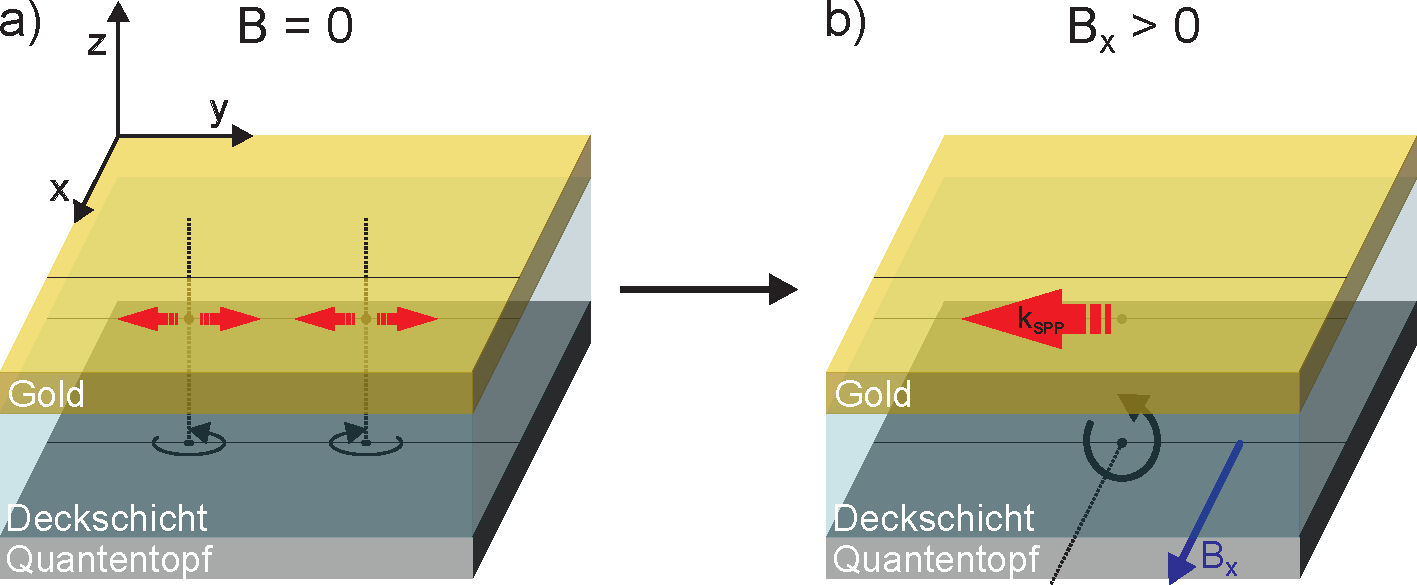
\includegraphics[scale=0.5]{./Plots/exziton.pdf}
    \caption{Darstellung von Exzitonen in unterschiedlichen Ebenen, bei gegebenen Magnetfeld.\\
    In a) befinden sich die Exzitonen mit ihrer Polarisation in der x-y-Ebene.\\
    In b) befinden sich die Exzitonen anteilig mit ihrer Polarisation in der y-z-Ebene.\cite{lars}}
    \label{fig:exziton}
\end{figure}
\FloatBarrier

Diese sich in der y-z-Ebene befindenden Exzitonen können im folgenden, an die in der Deckschicht sich bildenden 
Plasmonen (SSP) mit gleichseitiger zirkularer Polarisation, koppeln.
\footnote{Bei der Umpolung des Magnetfelds kehrt sich der Drehsinn der Polarisation um  
Die Aussage, dass Exzitonen zirkular Polarisiert sind eher ungenau, denn die Polarisation
ist eine Eigenschaft des Lichtes bei der Rekombination zwischen Elektron und Loch.}
Aus dem Grund koppeln linkszirkulare Exzitonen mit linkszirkularen Plasmonen und 
rechtszirkulare Exzitonen mit rechtszirkularen Plasmonen.

Bei anliegendem konstanten Magnetfeld liegt eine Vorzugspolarisation unter 
den entstanden Exzitonen, bedingt durch die Schwerlochband-Übergänge, vor.
% das ausgesendete licht ist p pol
Sodass beispielsweise Anteilig deutlich mehr rechtszirkulare Exzitonen existieren
als linkszirkulare. 
Diese Differenz pflanzt sich in die Entstehung der Plasmonen (SPPs) fort.
Das sich auf der Oberfläche der Probe befindende Goldgitter, sorgt wie in Abschnitt~\ref{sec:spps}
beschrieben dafür, dass die SPPs in Photonen emittieren können und die Probe als PL verlassen.
Die gebildete Vorzugspolarisation sorgt bei diesem Prozess für eine ebenfalls bevorzugte Emittierung von Photonen
in eine Richtung. 
Dieser Effekt wird als transversale magnetische Führung der Lichtemission 
(engl. transverse magnetic routing of light emission, TMRLE) bezeichnet.

Wird die Temperatur der Probe um wenige Kelvin gesteigert, ist eine Abschwächung des Effekt zu erkennen.
Die Größe $\Delta_\text{h,F}(T)$ in Gleichung~\ref{eq:pc} ist Temperaturabhängig. 
Die Temperatur sorgt dafür, dass sich die Spins der Exzitonen schlechter entlang
des Magnetfelds ausrichten können.\cite{felix}